\documentclass[10pt]{article}

\usepackage[margin=0.85in]{geometry}
\usepackage{amsmath}
\usepackage{booktabs}
\usepackage{graphicx}
\usepackage{microtype}
\usepackage[numbers,sort&compress]{natbib}
\usepackage{xurl}
\usepackage[hidelinks]{hyperref}

\title{FoldPipe: Bounded Remote Streaming of Native Molecular-Graph Shards\\
with Conditional I/O--Compute Overlap}
\author{Dhiren Mukesh Khatri\\
\small Independent Researcher}
\date{Draft of August 17, 2026}

\begin{document}
\maketitle

\begin{abstract}
Training atomistic neural networks on ephemeral or memory-constrained
accelerator instances can require retrieving preprocessed molecular graphs from
remote storage.  FoldPipe is a lightweight Python orchestration layer that
iterates over native PyTorch/PyTorch Geometric shard files, retrieves one shard
ahead in a background thread, and keeps a constant-number shard working set.
The prefetch principle is established systems practice rather than a new
scheduling algorithm; the contribution here is a compact molecular-data
integration and a source-pinned empirical characterization of when its overlap
does and does not translate into wall-clock improvement.

We evaluate a SchNet energy-and-force training step on MD17 aspirin data using
20 paired, order-alternating passes on a Kaggle Tesla T4.  Each pipeline pass
retrieves five revision-pinned shards containing 25,000 structures in total.
FoldPipe directly recorded 16.33 s mean overlap between shard retrieval and
training, compared with 0 s by construction for the sequential bounded
baseline.  Mean pass time was 76.78 s for FoldPipe and 83.37 s for the
baseline.  However, the primary paired estimate was only 1.0587$\times$
geometric-mean speedup with a 95\% bootstrap interval of
0.8776$\times$--1.2880$\times$; intervals for paired time savings also crossed
zero.  The experiment therefore demonstrates operation of the overlap
mechanism but is inconclusive about a speed advantage under the observed
public-network variability.  This negative statistical result delineates the
system's useful regime: prefetch can hide only the portion of retrieval that
coincides with current-shard computation.
\end{abstract}

\section{Introduction}

Molecular machine-learning workloads commonly represent each conformation as a
small graph carrying atomic numbers, coordinates, energies, and forces.  Model
implementations such as SchNet~\cite{schutt2018schnet} can consume these objects
through PyTorch Geometric (PyG)~\cite{fey2019pyg}, but dataset preparation and
deployment choices still determine whether an accelerator receives batches on
time.  On a temporary notebook runner, a processed corpus may live in remote
object storage rather than on a fast local filesystem, while the complete
corpus may be larger than the runner's memory or persistent disk budget.

General-purpose solutions already cover much of this design space.  PyTorch
provides multiprocessing data loading~\cite{paszke2019pytorch}; PyG provides
database-backed on-disk datasets and host-to-device prefetch
utilities~\cite{pygondiskdocs,pygloaderdocs}; Hugging Face provides
revision-addressable remote repository storage and file
retrieval~\cite{huggingfacehub}; and WebDataset uses streaming tar
shards~\cite{aizman2020webdataset}.  Larger systems optimize preprocessing,
caching, and out-of-core graph access at substantially greater scope
\cite{murray2021tfdata,mohan2021stalls,graur2022cachew,waleffe2023mariusgnn}.
FoldPipe does not replace these systems.

Instead, FoldPipe targets a narrower migration problem: a researcher already
has bounded-size \texttt{.pt} shards containing native tensor or PyG objects and
wants to consume them directly from Hugging Face or Google Drive without first
re-encoding them into tar records or a database.  FoldPipe adds a two-method
source interface and a one-stage producer--consumer loop around those files.
Its scientific value depends less on algorithmic novelty than on stating the
performance boundary correctly and publishing enough timing provenance to test
it.

This paper makes three contributions:

\begin{enumerate}
  \item It describes a small, backend-independent integration for remote,
  native PyTorch/PyG shards whose number of live shard payloads is constant in
  the total dataset size.
  \item It provides a traceable paired benchmark protocol that records source
  and data revisions, pipeline order, per-shard transfer and training
  intervals, payload bytes, memory, utilization samples, and raw paired
  outcomes.
  \item It reports a scientifically conservative real-network result: overlap
  is observed, but a throughput advantage is not statistically established in
  20 paired MD17/SchNet passes.
\end{enumerate}

No claim is made that asynchronous prefetch, bounded buffering, or the ideal
two-stage overlap equation is novel.

\section{Background and Related Work}

\subsection{Prefetch and ML input pipelines}

Overlapping input with computation predates contemporary machine learning.
Shriver, Small, and Smith analyzed why filesystem prefetch works and explicitly
identified computation--I/O overlap as one source of throughput improvement
\cite{shriver1999prefetching}.  The familiar result that equal-duration stages
can approach a twofold throughput improvement is therefore prior art, not a
FoldPipe contribution.

Modern ML frameworks broaden the same principle.  The \texttt{tf.data}
runtime composes parallelism, caching, and input transformations while
overlapping communication and computation~\cite{murray2021tfdata}.  CoorDL
analyzes fetch and preprocessing stalls and coordinates preprocessing and
caching~\cite{mohan2021stalls}.  FFCV combines a dedicated format, caching,
preloading, asynchronous transfer, and compilation~\cite{leclerc2023ffcv}.
OneAccess argues for cluster-wide sharing across jobs
\cite{kakaraparthy2019oneaccess}, while Cachew adds managed resource scaling and
caching~\cite{graur2022cachew}.  These systems pursue throughput, sharing, and
automatic optimization beyond FoldPipe's scope.

\subsection{Formats, remote streaming, and graph systems}

WebDataset packages samples into tar shards designed for sequential streaming
from local or remote storage~\cite{aizman2020webdataset}. The Hugging Face Hub
provides revision-addressable repository storage and remote file
retrieval~\cite{huggingfacehub}. FoldPipe uses that storage boundary to
retrieve native \texttt{.pt} shards directly. FoldPipe's distinction is compatibility,
not superior generality: it accepts already-produced \texttt{.pt} shard objects
without a separate format migration.  This also gives up capabilities such as
sample-level streaming within a shard, rich transformation graphs, automatic
shuffle, and mature distributed partitioning.

PyG's \texttt{OnDiskDataset} stores graph objects through a database backend
when they do not fit in CPU memory~\cite{pygondiskdocs}, and its
\texttt{PrefetchLoader} asynchronously transfers prepared batches from host to
device~\cite{pygloaderdocs}.  FoldPipe acts at a different boundary: remote
file retrieval and deserialization before PyG batching.  For single massive
graphs, MariusGNN pipelines across the memory/storage hierarchy
\cite{waleffe2023mariusgnn}, and Helios uses GPU-initiated asynchronous SSD I/O
and heterogeneous caching~\cite{sun2023helios}.  FoldPipe is not a competitor
to those graph-partitioning systems; its shards contain many independent small
molecular graphs.

\subsection{Molecular workload}

The evaluation uses the aspirin trajectory from MD17, introduced with
gradient-domain molecular force fields~\cite{chmiela2017md17}, transformed by
PyG into graph objects.  SchNet's continuous-filter architecture provides the
energy model used in each timed optimization step~\cite{schutt2018schnet}.  The
paper evaluates data-path behavior, not a new molecular representation, force
field, or accuracy result.

\section{FoldPipe Design}

\subsection{Source abstraction}

A \texttt{Source} exposes two operations: a lazy iterator over shard
identifiers and a function that retrieves and deserializes one identifier.
The release contains Hugging Face, Google Drive, controlled-latency, and
pre-enumerated sources.  Backend discovery is separated from consumption so a
benchmark may freeze its shard list before starting a timed pass.

The Hugging Face implementation requests a revision-specific file, streams the
response into an in-memory byte buffer, and deserializes it on the CPU.  This
avoids a local-disk cache and a separate dataset-format conversion.  It is not
zero-copy: the serialized bytes and deserialized objects can coexist briefly.
Moreover, the current implementation calls \texttt{torch.load} with
\texttt{weights\_only=False}; shards must therefore come from a trusted source.

\subsection{One-stage prefetch}

The consumer submits retrieval of the first shard to a single-worker thread
pool.  After waiting for shard $i$, it immediately submits shard $i+1$ and then
yields batches from shard $i$ to the training loop.  When the current shard is
exhausted, the consumer waits only for any unfinished portion of the next
future.

For $n$ shards, let $D_i$ be retrieval plus deserialization time and $C_i$ the
time consuming shard $i$.  Ignoring small orchestration overheads, the
sequential bounded path has

\begin{equation}
T_{\mathrm{seq}} = \sum_{i=1}^{n}(D_i + C_i),
\end{equation}

whereas an ideal one-stage pipeline has

\begin{equation}
T_{\mathrm{pipe}} = D_1 +
\sum_{i=1}^{n-1}\max(C_i, D_{i+1}) + C_n.
\end{equation}

In a homogeneous long stream this approaches per-shard time
$\max(D,C)$ instead of $D+C$.  The model explains two important limits.  First,
startup and drain cannot be hidden.  Second, if retrieval is much slower than
computation, only $C$ of each later retrieval can be masked.  These are standard
pipeline properties~\cite{shriver1999prefetching,murray2021tfdata}, included to
interpret measurements rather than claimed as a new result.

\subsection{Memory invariant}

Shard identifiers are produced lazily.  At steady state, the main thread can
hold the current deserialized shard while the future holds the next shard or
its in-progress byte buffer.  Mini-batch objects add a smaller workload-specific
term.  If every shard is bounded by $S_{\max}$, the live data-path memory is
$O(S_{\max})$ and independent of the total shard count, with a constant factor
that can approach two shard payloads.  FoldPipe therefore does not promise
``one shard exactly,'' zero memory, or immunity to out-of-memory failures from
an individually oversized shard.

\section{Experimental Method}

\subsection{Workload and environment}

The released experiment ran on a Kaggle Tesla T4.  It retrieved five private
Hugging Face shards derived from PyG's MD17 \texttt{aspirin} dataset.  Each
shard contains 5,000 graph objects, so one timed pass processes 25,000
structures.  The shard list was fixed before timing and the dataset repository
was pinned to revision
\texttt{f779686deb9217877dd7ddde99b2522bd441492a}.

The model was PyG SchNet with 128 hidden channels, 128 filters, six interaction
blocks, 50 Gaussian basis functions, and a 10~\AA{} cutoff.  A batch contains
32 molecular graphs.  Each step predicts energy, obtains forces as the negative
position gradient, and optimizes an energy mean-squared error plus ten times
the force mean-squared error.  The model received one untimed warm-up batch.

\subsection{Paired protocol}

The experiment formed 20 pairs.  Within each pair, both the sequential bounded
stream and FoldPipe processed the same five shards from the same initial model
state and manual seed.  Execution order alternated by pair to distribute
time-varying network conditions: sequential then FoldPipe for even-indexed
pairs, and the reverse for odd-indexed pairs.  This yielded 40 timed passes,
200 shard traces, and 1,000,000 repeated structure-visits.  The last quantity
must not be interpreted as one million unique structures.

The benchmark used monotonic timestamps for download start, download finish,
deserialization finish, training start, and training finish.  Resident set size
and GPU utilization from \texttt{nvidia-smi} were sampled every 0.5 s.  GPU
synchronization delimited each shard's training interval.  Discovery overhead
was excluded by the fixed shard list, while each timed pass still retrieved and
deserialized every payload.

The primary multiplicative estimand is the geometric mean of the 20 paired
ratios $T_{\mathrm{seq}}/T_{\mathrm{FoldPipe}}$.  Its 95\% interval is a
deterministic percentile bootstrap of paired log ratios with 20,000 resamples.
Paired arithmetic time savings and their median are secondary estimands with
paired percentile-bootstrap intervals.  Pipeline-specific means are reported
descriptively.  The full raw traces and seeds are included in the v0.3.0
artifact~\cite{khatri2026foldpipe}.

The executed source tree was clean commit
\texttt{16fdbb26b00f9721ce4034335ce0ee12bda77720}.  A source manifest records a
bundle SHA-256 of
\texttt{4fc3f6d712557822efc0d5d71aaa616b0fe30f578631726ef60d6a0fe73b32c0}.

\section{Results}

\begin{table}[t]
\centering
\caption{Twenty-pair MD17/SchNet summary.  Pipeline-specific means are
descriptive; inference about runtime uses the paired effects below.}
\label{tab:results}
\begin{tabular}{lrr}
\toprule
Metric & Sequential & FoldPipe \\
\midrule
Mean pass time (s) & 83.37 & 76.78 \\
Median pass time (s) & 75.27 & 75.97 \\
Time standard deviation (s) & 39.86 & 28.46 \\
Mean sampled GPU utilization (\%) & 36.17 & 37.70 \\
Mean peak RSS (GiB) & 1.935 & 2.064 \\
Mean I/O--compute overlap (s) & 0.00 & 16.33 \\
Mean measured GPU wait (s) & 56.50 & 48.65 \\
\bottomrule
\end{tabular}
\end{table}

FoldPipe was faster in 11 of 20 pairs.  The geometric mean paired speedup was
1.0587$\times$, but its 95\% interval was
0.8776$\times$--1.2880$\times$.  Mean paired time saved was 6.59 s with a 95\%
interval of $-7.69$ to 21.11 s.  Median paired time saved was 3.45 s with an
interval of $-13.48$ to 22.89 s.  All three intervals include their respective
no-effect values, so this experiment is inconclusive about a wall-clock speed
advantage.

The mechanism measurement answers a different question.  FoldPipe recorded
16.33 s mean overlap per pass (95\% pipeline-specific bootstrap interval
15.04--17.70 s), whereas the sequential implementation has no concurrent
retrieval and training by construction.  Thus the implementation did execute
the intended overlap.  That overlap was insufficient to overcome large
between-pass network variation reliably in this sample.

Peak RSS was higher for FoldPipe by 0.129 GiB in the unpaired mean summary,
which is consistent with retaining a prefetched next payload.  The experiment
does not support a claim that asynchronous execution uses less memory than the
sequential bounded stream; both hold a constant number of shards.  Likewise,
the 1.53 percentage-point difference in sampled mean GPU utilization is treated
as descriptive rather than statistically established.

\begin{figure}[t]
  \centering
  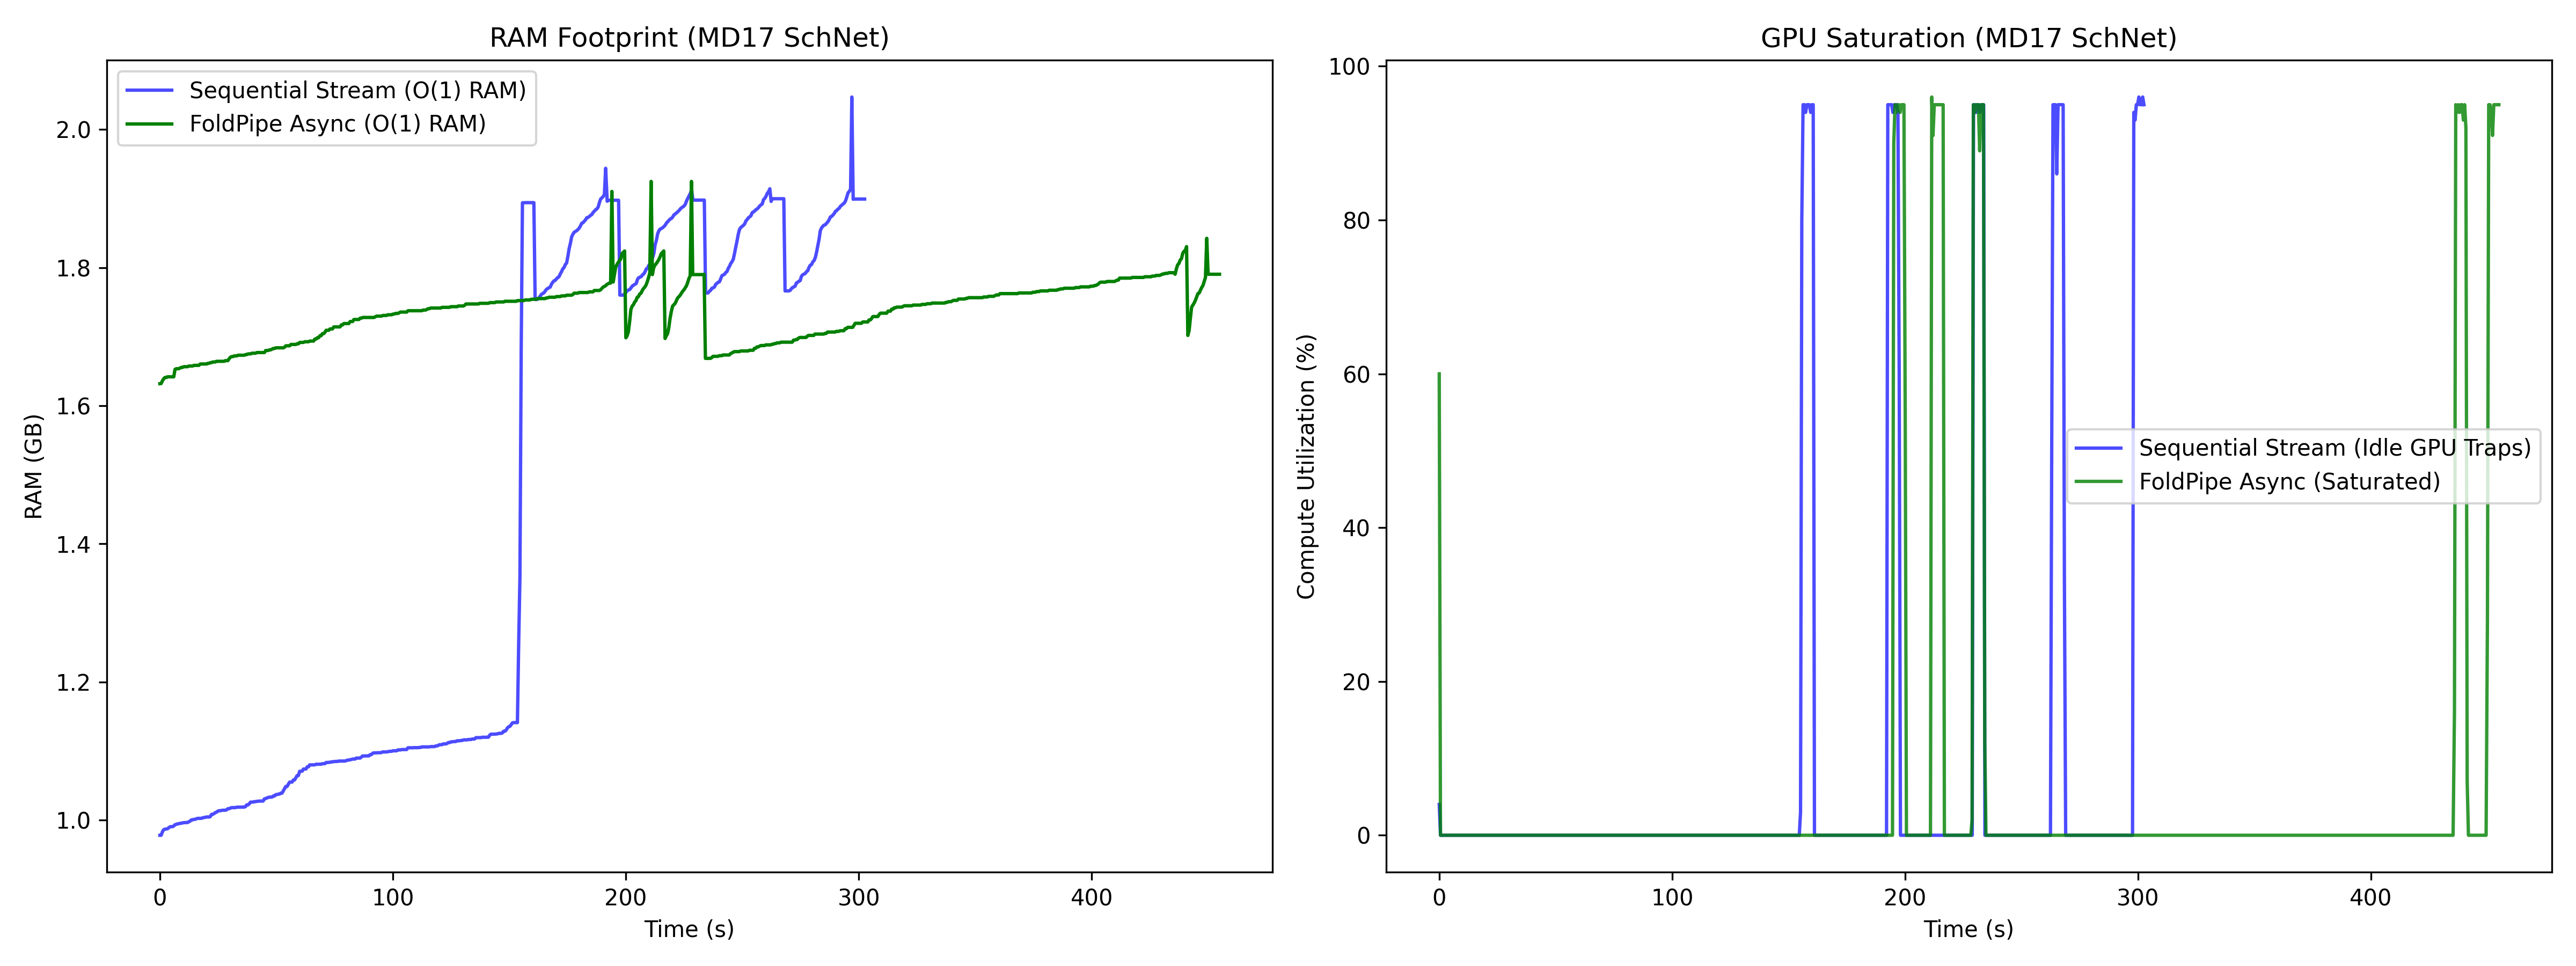
\includegraphics[width=\linewidth]{../results/benchmark_comparison_md17.png}
  \caption{Resident memory and sampled GPU utilization for the first recorded
  pass of each pipeline.  These representative traces illustrate bursty
  execution but are not the basis of the paired runtime inference.}
  \label{fig:representative}
\end{figure}

\section{Discussion}

The result separates mechanism from outcome.  A completed future proves that
some retrieval occurred during current-shard training; it does not guarantee a
shorter pass when $D_i$ varies sharply across a public network.  FoldPipe's
benefit should be largest when current-shard computation is comparable to the
next retrieval, when enough of $D_{i+1}$ can be hidden without leaving the
consumer waiting.  In an I/O-dominant regime, a depth-one queue cannot conceal
the excess retrieval time.  In a compute-dominant regime, retrieval can be
mostly hidden, but the total gain is then bounded by a relatively small I/O
fraction.

The engineering trade-off is similarly conditional.  Researchers who already
possess native, trusted \texttt{.pt} shards can avoid a conversion stage and
retain PyG object semantics.  Researchers optimizing stable cluster-scale
throughput may prefer WebDataset, FFCV, a database-backed PyG dataset, or a
storage-aware graph system.  FoldPipe currently offers neither their breadth
nor their optimization depth.

\section{Limitations and Threats to Validity}

\paragraph{Single environment and dataset slice.}
The real experiment uses one Kaggle T4, one model configuration, the first five
aspirin shards, and one public remote service.  It does not establish results
for other accelerators, molecules, regions, object stores, or heavier
equivariant models.

\paragraph{Repeated and temporally correlated observations.}
The same 25,000 structures are revisited in every pass.  Network conditions can
remain correlated across adjacent pairs, while the percentile bootstrap treats
pairs as exchangeable.  Twenty pairs leave a wide interval.  Alternating order
reduces a simple first-run bias but is not full randomization or a time-series
model.

\paragraph{Telemetry resolution.}
GPU utilization is a coarse 0.5 s sample from \texttt{nvidia-smi}, not a kernel
trace.  Process RSS omits some external allocations and does not prove an
asymptotic memory bound empirically.  The bound follows from the live-object
invariant under a bounded maximum shard size.

\paragraph{Pipeline scope.}
There is one prefetch worker and no adaptive queue depth, local persistent
cache, retry/checkpoint protocol, distributed partitioning, random access, or
sample-level shuffle.  A very large shard can still exhaust memory.  Python
object deserialization may be significant and is unsafe for untrusted
artifacts.

\paragraph{Scientific scope.}
The benchmark times optimization steps but does not report validation error,
force accuracy, convergence, or simulation stability.  It is a systems
benchmark over an established molecular workload, not evidence of a better
molecular potential.

\paragraph{Dataset metadata.}
The private Hugging Face mirror is revision-pinned, but at the time of writing
it lacks a dataset card and explicit license metadata.  The repository's
migration script traces it to PyG's original MD17 aspirin loader; nevertheless,
the mirror must receive an upstream citation, transformation description, and
verified redistribution license before public artifact release or manuscript
submission.

\section{Reproducibility and Research Integrity}

The GitHub release contains raw JSON for every pair and shard, a generated
report, plot, execution log, and source manifest.  The Kaggle artifact records
the exact data revision and executed code bundle.  The repository is MIT
licensed~\cite{khatri2026foldpipe}.  The current software release is FoldPipe
0.3.2; the MD17 measurements analyzed here are preserved in the frozen v0.3.0
research artifact.

The manuscript deliberately attributes prefetching and input pipelining to
prior work, uses no third-party figure, and reports the inconclusive paired
intervals alongside point estimates.  A separate repository audit documents
public-code phrase searches, commit provenance, claim boundaries, and remaining
dataset-license work.  Before submission, the rendered manuscript should also
be checked with the target institution's publisher-corpus similarity service;
public-web searches cannot provide equivalent coverage.

\section{Conclusion}

FoldPipe is a compact adapter for a specific deployment path: remote,
already-sharded, native molecular graph objects on constrained compute.  Its
one-stage background fetch creates measurable I/O--compute overlap while
keeping the number of live shards independent of total dataset size.  In the
released 20-pair MD17/SchNet study, the mechanism operated as designed, but
network variability left the runtime effect unresolved.  The defensible claim
is therefore conditional: FoldPipe can hide the portion of next-shard
retrieval concurrent with current-shard computation; it does not guarantee
acceleration.  Broader performance claims require controlled multi-seed
crossover experiments and additional real environments.

\bibliographystyle{unsrtnat}
\bibliography{references}

\end{document}

